\section{停止条件与计算成本}
\label{sec:saddle-stopping}

算法什么时候可以停，一次运行究竟可以报告什么？第~\ref{chap:smooth-foundations}章要求比较算法之前固定三件事：误差标准、返回哪个点、计算量怎样累计。这里把这三件事放到二阶情形下落实。

\paragraph{两个容差}
只有一个梯度容差无法排除鞍点，所以要同时控制梯度大小和Hessian最小特征值的负部。

\begin{definition}[近似二阶驻点]
 \label{def:saddle-approximate}
 给定$\varepsilon_g>0$，$\varepsilon_H>0$，若点$\bm{x}$满足
 \begin{equation}
  \lVert\nabla f(\bm{x})\rVert_2\leq\varepsilon_g,\qquad
  \lambda_{\min}\bigl(\nabla^2f(\bm{x})\bigr)\geq-\varepsilon_H,
  \label{eq:saddle-approximate}
 \end{equation}
 就称它为$(\varepsilon_g,\varepsilon_H)$\term{近似二阶驻点}（approximate second-order stationary point）。
\end{definition}

例中$\varepsilon_g=0.1$，$\varepsilon_H\approx0.775$。点$(0,0.0625)$的梯度范数$0.0625$通过了第一个条件，$\lambda_{\min}=-1$没有通过第二个。点$(0.9686,0.0039)$的梯度范数$0.060$，$\lambda_{\min}=1$，两个都通过。图~\ref{fig:saddle-tolerance-plane}(a)把表~\ref{tab:saddle-nc-run}的运行画在这两个量组成的平面上，(b)在变量空间中画出了两种验收区的差别。

\begin{BookInlineFigure}
  \centering
  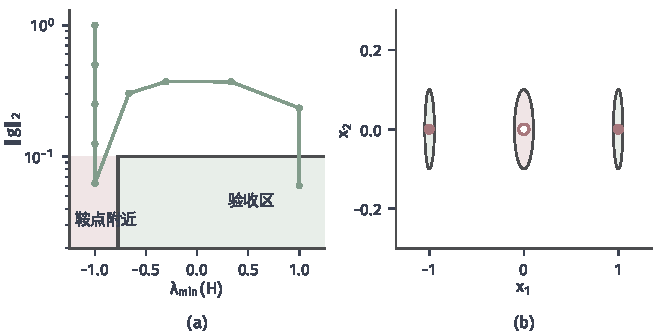
\includegraphics[width=112mm]{figures/05-optimization/02-smooth-optimization/matplotlib/saddle-tolerance-plane/figure.pdf}
  \caption{两个容差的验收区，$\varepsilon_g=0.1$，$\varepsilon_H\approx0.775$。(a)横轴是$\lambda_{\min}(\bm{H})$，纵轴是$\lVert\bm{g}\rVert_2$（对数坐标），绿色矩形是验收区，粗线是边界，浅红区梯度合格而曲率不合格，折线是表~\ref{tab:saddle-nc-run}的运行。(b)目标~\eqref{eq:saddle-example}上$\lVert\nabla f\rVert_2\leq\varepsilon_g$的三块区域，鞍点周围的一块（浅红）不满足曲率条件，只有两侧（浅绿）满足全部条件。}
  \label{fig:saddle-tolerance-plane}
\end{BookInlineFigure}

\paragraph{两个容差怎样搭配}
两个容差不是独立的。式~\eqref{eq:saddle-approximate}对目标下降的限制可以由三次上界直接算出：设半径$r$的球落在引理~\ref{lem:saddle-cubic}的凸集内，对$\lVert\bm{p}\rVert_2\leq r$，由该引理和式~\eqref{eq:saddle-approximate}，
\begin{equation}
 f(\bm{x}+\bm{p})\geq f(\bm{x})-\varepsilon_gr-\frac12\varepsilon_Hr^2-\frac{M}{6}r^3.
 \label{eq:saddle-tolerance-drop}
\end{equation}

三项分别来自梯度、负曲率和Hessian的变化。让三项同量级，由后两项得到$r\sim\varepsilon_H/M$，代入前两项得到$\varepsilon_g\sim\varepsilon_H^2/M$，于是自然的搭配是
\begin{equation}
 \varepsilon_H=\sqrt{M\varepsilon_g}.
 \label{eq:saddle-tolerance-scale}
\end{equation}

此时取$r=\sqrt{\varepsilon_g/M}$，式~\eqref{eq:saddle-tolerance-drop}的三项合计给出
\[
 f(\bm{x}+\bm{p})\geq f(\bm{x})-\frac{5}{3}\frac{\varepsilon_g^{3/2}}{\sqrt{M}}.
\]
这就是通过验收的点能保证的事：在半径$r$的球内，目标至多还能下降这么多。

\paragraph{通过验收不等于局部极小}
式~\eqref{eq:saddle-tolerance-drop}只限制了小球内的下降幅度，并不排除下降。$x_1^2-x_2^4$在原点梯度和Hessian的负部都是零，对任意容差都通过验收，而原点不是局部极小点，甚至这个目标没有下界。

容差取得过大也会放过严格鞍点。例中若$\varepsilon_H=2$，原点的$\lambda_{\min}=-1$就能通过。

所以报告结果时，应该写“近似二阶驻点，容差为$(\varepsilon_g,\varepsilon_H)$”，不写“找到了局部极小点”，更不写“找到了最优解”。

\paragraph{返回哪个点}
验收条件是针对具体的点的，所以返回的点必须就是验收的那个点。负曲率算法直接返回验收通过的$\bm{x}^{(t)}$。扰动梯度法返回窗口开始之前保存的基点$\tilde{\bm{x}}$，因为梯度小的判断是在基点上作出的，窗口结束时的点没有经过判断。

\paragraph{要累计哪些计算量}
这一节的成本有四类，单位要分开：梯度次数，Hessian向量积次数，矩阵分解次数，以及扰动窗口的梯度次数。

扰动窗口的次数也有上界。除了最后一次之外，每次窗口都使目标下降至少$F$，所以窗口总数不超过$\Delta_f/F+1$。例中上界是$16$次窗口，共$304$次梯度，实际只用了$2$次窗口。每次窗口都有失败的可能，失败概率要像下面的检测一样累计。

检测的失败概率也要累计。负曲率算法可能进行多次检测，任何一次“未找到”判断错误都会使算法提前停止。若检测次数不超过$K$，每次失败概率取$\delta/K$，由并的概率不等式，总失败概率不超过$\delta$，代价只是对数因子$\ln(K/\delta)$。

检测有两个方向，失败只发生在“未找到”的方向上。每次发现负曲率都是确定的，所以不需要担心算法走错一步。真正的风险是错误地宣布停止。下面把这些成本组合起来。

取$\gamma_0=\varepsilon_H/2$，检测精度$\varepsilon_H/2$，由式~\eqref{eq:saddle-no-find}，未找到时$\lambda_{\min}\geq-\varepsilon_H$。把$\varepsilon_H=\sqrt{M\varepsilon}$代入定理~\ref{thm:saddle-nc-count}，负曲率步的次数不超过
\begin{equation}
 K=\frac{12\sqrt{M}\,\Delta_f}{\varepsilon^{3/2}}.
 \label{eq:saddle-detect-count}
\end{equation}

用Lanczos方法时每次检测$O(\sqrt{L/\varepsilon_H}\,\ln(nK/\delta))$次乘积，总数是
\begin{equation}
 O\Bigl(\frac{\sqrt{L}\,M^{1/4}\Delta_f}{\varepsilon^{7/4}}\ln\frac{nK}{\delta}\Bigr).
 \label{eq:saddle-lanczos-total}
\end{equation}
这个量对$1/\varepsilon$的幂次比梯度步的$O(L\Delta_f/\varepsilon^2)$低$1/4$，所以在小容差下乘积的总量不会超过梯度的总量。换成幂迭代时，每次检测$O((L/\varepsilon_H)\ln(nK/\delta))$次乘积，总数变成$O((L\Delta_f/\varepsilon^2)\ln(nK/\delta))$，与梯度步同阶。

表~\ref{tab:saddle-cost-bounds}汇总了各种做法在最坏情形下的曲率成本，表中$\varepsilon_g=\varepsilon$，$\varepsilon_H=\sqrt{M\varepsilon}$。前三行的梯度次数都不超过$2L\Delta_f/\varepsilon^2$加检测带来的少量读取，扰动梯度法的梯度次数是$\tilde O(L\Delta_f/\varepsilon^2)$，这里的$\tilde O$隐去了对数因子。

\begin{BookInlineTable}
  \centering
  \begin{tabular}{@{}lll@{}}
    \toprule
    方法 & 曲率读取（梯度次数见正文） & 保证\\
    \midrule
    梯度下降 & 无 & 一阶，确定\\
    负曲率步，特征分解 & $O(\sqrt{M}\Delta_f/\varepsilon^{3/2})$次分解 & 二阶，确定\\
    负曲率步，Lanczos & 式~\eqref{eq:saddle-lanczos-total}的次数 & 二阶，$\geq1-\delta$\\
    扰动梯度法 & 无 & 二阶，$\geq1-\delta$\\
    信赖域，精确子问题 & $O(\varepsilon^{-2})$轮，每轮一次分解 & 二阶，确定\\
    \bottomrule
  \end{tabular}
  \caption{达到式~\eqref{eq:saddle-approximate}的最坏情形成本，“二阶”指近似二阶驻点，“$\geq1-\delta$”指成立的概率。信赖域一行由第~\ref{chap:trust-region}章的轮数估计得到，并依赖半径下界中的常数。}
  \label{tab:saddle-cost-bounds}
\end{BookInlineTable}

\paragraph{一次实际运行的账}
上界比较的是最坏情形，单次运行要按实际次数报告。表~\ref{tab:saddle-run-cost}是从$(0,1)$出发、$\varepsilon_g=0.1$、$\varepsilon_H\approx0.775$时各方法的实际计数。

\begin{BookInlineTable}
  \centering
  \begin{tabular}{@{}lrlcc@{}}
    \toprule
    方法 & 梯度 & 曲率读取 & 返回点 & 通过\\
    \midrule
    梯度下降 & $5$ & 无 & $(0,\ 0.0625)$ & 否\\
    谱修正Newton & $2$ & $1$次分解 & $(0,\ 0)$ & 否\\
    信赖域，截断CG & $2$ & $1$次乘积 & $(0,\ 0)$ & 否\\
    负曲率步，特征分解 & $10$ & $2$次分解 & $(0.969,\ 0.004)$ & 是\\
    负曲率步，幂迭代 & $11$ & $151$次乘积 & $(0.981,\ -0.001)$ & 是\\
    扰动梯度法 & $44$ & 无 & $(1.000,\ 0.000)$ & 是\\
    信赖域，精确子问题 & $3$ & $3$次分解 & $(1.039,\ 0)$ & 是\\
    \bottomrule
  \end{tabular}
  \caption{从$(0,1)$出发的实际计数，“通过”指是否满足式~\eqref{eq:saddle-approximate}。幂迭代用$L=2$，随机起点的种子固定为$0$，检测精度$\varepsilon_H/2$，失败概率$\delta=0.05$（两次检测的总失败概率约$0.1$），上限由式~\eqref{eq:saddle-power-rounds}算得$149$次。}
  \label{tab:saddle-run-cost}
\end{BookInlineTable}

表中前三行的算法都很便宜，但报告的点是鞍点。它们的共同问题是起点在$x_2$轴上，梯度始终看不到$x_1$方向。负曲率步用幂迭代时，第一次检测只用$2$次乘积就找到了方向，其余$149$次全部花在最后一次“未找到”的确认上。

这说明确认“没有负曲率”才是最贵的一步，手段越便宜，这一步越依赖概率。实际程序常常把上限设得比理论值小，这时要如实报告：这样的结果只是经验判断，不再带有定理~\ref{thm:saddle-power}的概率保证。

\paragraph{一次报告应该包含什么}
把三件事落实到底，一次运行的结论可以写成这样：对目标~\eqref{eq:saddle-example}，从$(0,1)$出发，用幂迭代检测负曲率的交替算法，返回点满足$\lVert\nabla f\rVert_2\leq0.1$；未找到负曲率的判断由$149$次乘积支持，至少以$0.9$的概率有$\lambda_{\min}\geq-0.775$；共用$11$次梯度和$151$次Hessian向量积。

这样的报告说清了误差标准（两个容差）、返回的点（验收通过的点）、成本（分类计数）和可信度（失败概率）。它没有声称局部极小，也没有声称全局最优，这两件事本章的方法都保证不了。

